% =====================================================================
% ITMA architecture diagram (standalone -> fig_arch.pdf)
% Compile:  pdflatex fig_arch.tex   (run from paper/figures/)
% Produces a tight, cropped PDF suitable for \includegraphics in any
% journal template (Springer sn-jnl, IEEEtran, ieeeaccess, elsarticle).
% Template-independent on purpose: built outside the main document so it
% does not collide with class-specific tikz/pgf settings.
% =====================================================================
\documentclass[border=4pt]{standalone}
\usepackage[T1]{fontenc}
\usepackage{amsmath,amssymb}
\usepackage{tikz}
\usetikzlibrary{arrows.meta,positioning,fit,backgrounds,calc,shapes.geometric}

\begin{document}
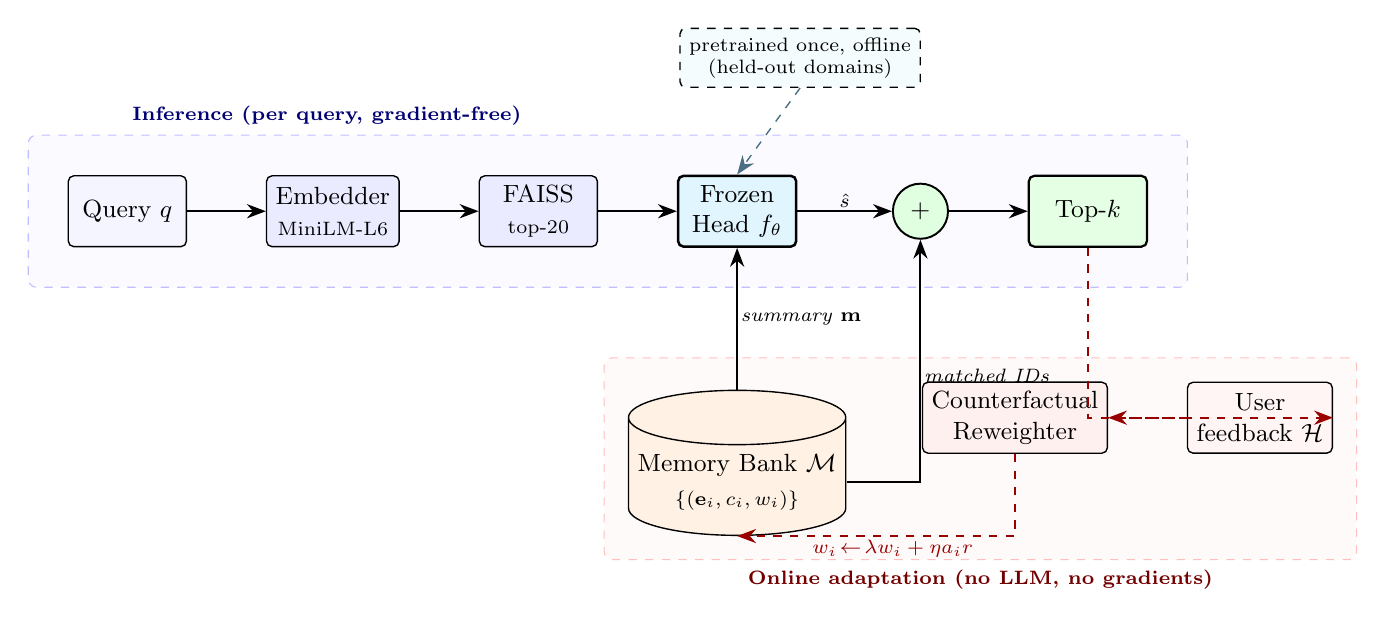
\begin{tikzpicture}[
    font=\small,
    >={Stealth[length=2.4mm]},
    node distance=10mm,
    block/.style={draw,rounded corners=2pt,minimum height=9mm,minimum width=15mm,
                  align=center,fill=blue!4,line width=0.5pt},
    proc/.style={block,fill=blue!8},
    frozen/.style={block,fill=cyan!12,line width=0.9pt},
    store/.style={draw,cylinder,shape border rotate=90,aspect=0.25,
                  minimum height=14mm,minimum width=22mm,align=center,fill=orange!10,line width=0.5pt},
    op/.style={draw,circle,minimum size=7mm,inner sep=0pt,fill=green!12,line width=0.7pt},
    outbox/.style={block,fill=green!10,line width=0.8pt},
    flow/.style={->,line width=0.7pt},
    fb/.style={->,line width=0.7pt,dashed,red!60!black},
    lbl/.style={font=\scriptsize\itshape,inner sep=1pt},
]

% ---- main horizontal retrieval pipeline (top row) ----
\node[block]            (q)     {Query $q$};
\node[proc,right=of q]  (emb)   {Embedder\\\scriptsize MiniLM-L6};
\node[proc,right=of emb](faiss) {FAISS\\\scriptsize top-20};
\node[frozen,right=of faiss] (head) {Frozen\\Head $f_\theta$};
\node[op,right=12mm of head] (boost) {$+$};
\node[outbox,right=10mm of boost] (top) {Top-$k$};

\draw[flow] (q)     -- (emb);
\draw[flow] (emb)   -- (faiss);
\draw[flow] (faiss) -- (head);
\draw[flow] (head)  -- node[lbl,above]{$\hat{s}$} (boost);
\draw[flow] (boost) -- (top);

% ---- memory bank (bottom) feeding both head and boost ----
\node[store,below=18mm of head] (mem)
     {Memory Bank $\mathcal{M}$\\[1pt]\scriptsize$\{(\mathbf{e}_i,c_i,w_i)\}$};

\draw[flow] (mem.north) -- node[lbl,right,pos=0.5]{summary $\mathbf{m}$} (head.south);
\draw[flow] (mem.east) -| (boost.south) node[lbl,right,pos=0.72]{matched IDs};

% ---- feedback / counterfactual reweighting loop ----
\node[proc,below=18mm of boost,xshift=12mm,fill=red!6] (rw)
     {Counterfactual\\Reweighter};
\node[block,right=10mm of rw,fill=red!4] (fbk) {User\\feedback $\mathcal{H}$};

\draw[fb] (top.south) |- (fbk.east);
\draw[fb] (fbk) -- (rw);
\draw[fb] (rw.south) |- (mem.south)
      node[lbl,below,pos=0.72]{$w_i\!\leftarrow\!\lambda w_i+\eta a_i r$};

% ---- offline pretraining note ----
\node[draw,dashed,line width=0.5pt,rounded corners=2pt,fill=cyan!4,
      align=center,font=\scriptsize,above=11mm of head,xshift=8mm] (off)
     {pretrained once, offline\\(held-out domains)};
\draw[->,line width=0.5pt,dashed,cyan!45!black] (off.south) -- (head.north);

% ---- grouping backgrounds ----
\begin{scope}[on background layer]
  \node[draw=blue!25,dashed,rounded corners=3pt,fill=blue!2,
        fit=(q)(emb)(faiss)(head)(boost)(top),inner sep=5mm,label={[font=\scriptsize\bfseries,blue!45!black]above left:Inference (per query, gradient-free)}] {};
  \node[draw=red!25,dashed,rounded corners=3pt,fill=red!2,
        fit=(mem)(rw)(fbk),inner sep=3mm,label={[font=\scriptsize\bfseries,red!45!black]below:Online adaptation (no LLM, no gradients)}] {};
\end{scope}

\end{tikzpicture}
\end{document}
